%%%%%%%%%%%%%%%%%%%%%%%%%%%%%%%%%%%%%%%%%%%%%%%%%%%%%%%%%%%%%%%%%%%%%%
% How to use writeLaTeX: 
%
% You edit the source code here on the left, and the preview on the
% right shows you the result within a few seconds.
%
% Bookmark this page and share the URL with your co-authors. They can
% edit at the same time!
%
% You can upload figures, bibliographies, custom classes and
% styles using the files menu.
%
%%%%%%%%%%%%%%%%%%%%%%%%%%%%%%%%%%%%%%%%%%%%%%%%%%%%%%%%%%%%%%%%%%%%%%

\documentclass[12pt]{article}

\usepackage{sbc-template}
\usepackage{bera}% optional: just to have a nice mono-spaced font
\usepackage{listings}
\usepackage{xcolor}
\usepackage{booktabs}
\usepackage{verbatim}
\usepackage{amsmath}
\usepackage{float}

\colorlet{punct}{red!60!black}
\definecolor{background}{HTML}{EEEEEE}
\definecolor{delim}{RGB}{20,105,176}
\colorlet{numb}{magenta!60!black}

\lstdefinelanguage{json}{
    basicstyle=\normalfont\ttfamily,
    numbers=left,
    numberstyle=\scriptsize,
    stepnumber=1,
    numbersep=8pt,
    showstringspaces=false,
    breaklines=true,
    frame=lines,
    backgroundcolor=\color{background},
    literate=
     *{0}{{{\color{numb}0}}}{1}
      {1}{{{\color{numb}1}}}{1}
      {2}{{{\color{numb}2}}}{1}
      {3}{{{\color{numb}3}}}{1}
      {4}{{{\color{numb}4}}}{1}
      {5}{{{\color{numb}5}}}{1}
      {6}{{{\color{numb}6}}}{1}
      {7}{{{\color{numb}7}}}{1}
      {8}{{{\color{numb}8}}}{1}
      {9}{{{\color{numb}9}}}{1}
      {:}{{{\color{punct}{:}}}}{1}
      {,}{{{\color{punct}{,}}}}{1}
      {\{}{{{\color{delim}{\{}}}}{1}
      {\}}{{{\color{delim}{\}}}}}{1}
      {[}{{{\color{delim}{[}}}}{1}
      {]}{{{\color{delim}{]}}}}{1},
}
\usepackage{graphicx,url}

\usepackage{graphicx}

\usepackage[brazil]{babel}   
\usepackage[utf8]{inputenc}  
\usepackage{geometry}
\usepackage{float}

\sloppy

\title{Parametrização e resolução do problema dos missionários e canibais}

\author{Jaime Antonio Daniel Filho\inst{1}, Diego Ribeiro Chaves\inst{1}}
\address{Curso de Ciência da Computação, Universidade Federal de Santa Maria
  (UFSM)\\
  \email{jafilho@inf.ufsm.br, drchaves@inf.ufsm.br}
}
\begin{document} 

\maketitle

\section{Introdução}

O problema dos missionários e canibais é um clássico da inteligência artificial e da teoria da busca. Na formulação original, três missionários e três canibais precisam atravessar um rio usando um barco com capacidade para duas pessoas, respeitando a restrição de que os canibais nunca podem superar em número os missionários em nenhum dos lados da margem, caso contrário, os missionários seriam devorados.

Neste trabalho, generalizamos o problema ao parametrizar o número de pares missionário-canibal como $N$ e a capacidade do barco como $K$. O objetivo é estudar como essas duas variáveis afetam a complexidade da busca: o número de estados explorados, o consumo de memória, o tempo de execução e a profundidade da solução ótima. A busca em largura (BFS) é utilizada por garantir que a primeira solução encontrada possui o menor número de movimentos possível.

\section{Metodologia}

Nesta seção, detalharemos a abordagem adotada para a modelagem, resolução e coleta de métricas do problema dos missionários e canibais. 

\subsection{Formulação do problema}

O problema foi formalizado utilizando estruturas de dados para representar os estados, que indicam a quantidade de canibais e missionários em cada margem e a posição do barco, em que, se um estado for considerado válido, é colocado em uma fila para ser explorado. A fila é explorada utilizando a abordagem FIFO, o que caracteriza o algoritmo de busca em largura (BFS).

\subsubsection{Estado inicial}

O espaço de estados é definido pela tripla $(L, C, M)$, onde:

\begin{itemize}
    \item $L \in \{0, 1\}$ indica em qual margem o barco está ($0$ = margem de origem, $1$ margem de destino);
    \item $C \in \{0, ..., N\}$ é o número de canibais na margem $L$;
    \item $M \in \{0, ..., N\}$ é o número de missionários na margem $L$.
\end{itemize}

O estado inicial é $(0, N, N)$, ou seja, todos os $N$ missionários e $N$ canibais estão na margem de origem, juntamente com o barco. Por outro lado, o estado final é $(1, N, N)$, ou seja, todos estão na margem de destino.

\subsubsection{Função sucessora}

A cada passo, o barco transporta entre $1$ e $K$ pessoas da margem onde ele se encontra para a outra. Os pares $(m, c)$ de missionários e canibais embarcados devem satisfazer:

\begin{itemize}
    \item $m + c \geq 1$ e $m + c \leq K$;
    \item Em ambas as margens, após a travessia, o número de missionários deve ser maior ou igual ao de canibais, a menos que não haja missionário algum naquela margem;
    \item Adicionalmente, adotamos a restrição de que dentro do próprio barco o número de missionários também deve ser maior ou igual ao de canibais, exceto quando não há missionários a bordo.
\end{itemize}

Como a função sucessora pode transicionar para um estado que já foi visto anteriormente, cada estado visto é armazenado em uma tabela \textit{hash}, comportamento que batizamos de deduplicação. Desse modo, um estado sucessor somente é adicionado à fila de avaliação, caso não for encontrado na tabela \textit{hash}. Isso impede que a BFS revisite os mesmos estados indefinidamente. A deduplicação é controlada pelo parâmetro $D$ ($0$ = desativado, $1$ = ativado). 

O caminho, isto é, as transições que foram realizadas para alcançar a solução é implementado por meio do \textit{backtracking}. A cada estado adicionado à fila, armazena-se o seu estado pai em outra tabela \textit{hash}. Ao final da execução, percorre-se a tabela de pais de trás para frente, buscando o pai do estado final $(1, N, N)$ até chegarmos no estado que possui o estado inicial $(0, N, N)$ como pai.

\subsection{Configurações testadas e métricas}

Os experimentos foram conduzidos variando:

\begin{itemize}
    \item $K$ de $1$ a $128$ em incrementos de $1$;
    \item $N$ de $1$ a $256$ em incrementos de $1$, e em seguida em progressão geométrica de base 2 até o consumo de memória exceder 4GB.
\end{itemize}

Para monitorar o desempenho e a evolução da busca, registrou-se um conjunto de métricas a cada nível de profundidade percorrido na árvore de estados. Essa abordagem permite observar o crescimento da fila e da tabela \textit{hash} de forma dinâmica, em vez de avaliar apenas o estado final.

A Tabela \ref{table:metricas} detalha os dados capturados em cada ponto de amostragem. A memória é estimada conforme a carga na estrutura da fila e na estrutura da tabela \textit{hash}.

\begin{table}[H]
\centering
\caption{Métricas registradas por nível de profundidade.}
\label{table:metricas}
\small
\begin{tabular}{p{3.5cm} p{11.5cm}}
\toprule
\textbf{Métrica} & \textbf{Descrição} \\
\midrule
\texttt{depth} & Profundidade atual da árvore de busca. \\
\texttt{queue size} & Número de estados na fila a serem avaliados. \\
\texttt{table size} & Número de estados armazenados pela tabela \textit{hash}. \\
\texttt{table buckets} & Número de baldes alocados pela tabela \textit{hash} \\
\texttt{states explored} & Número cumulativo de estados avaliados. \\
\texttt{states skipped} & Número de estados ignorados por já terem sido vistos. \\
\texttt{memory usage} & Estimativa do consumo de memória em bytes. \\
\texttt{time elapsed} & Tempo decorrido em nanosegundos. \\
\bottomrule
\end{tabular}
\end{table}

Abaixo é apresentado um formato de amostra da saída padronizada. O formato de resultado inicia sempre com os parâmetros utilizados e finaliza com o número de travessias mínimas para a solução.

\begin{tiny}
\begin{verbatim}
n: 128, k: 64, deduplicate: 1, memory limit: 4294967296

depth: 1, queue size: 95, table size: 97, table buckets: 127, states explored: 1, states skipped: 0, memory usage: 10566, time elapsed: 32940
depth: 2, queue size: 93, table size: 191, table buckets: 257, states explored: 97, states skipped: 3042, memory usage: 16410, time elapsed: 56101
depth: 3, queue size: 93, table size: 285, table buckets: 541, states explored: 191, states skipped: 9027, memory usage: 26046, time elapsed: 232473
depth: 4, queue size: 93, table size: 379, table buckets: 541, states explored: 285, states skipped: 14484, memory usage: 28866, time elapsed: 304448
depth: 5, queue size: 31, table size: 411, table buckets: 541, states explored: 379, states skipped: 17524, memory usage: 26850, time elapsed: 449746
depth: 6, queue size: 31, table size: 443, table buckets: 541, states explored: 411, states skipped: 18549, memory usage: 27810, time elapsed: 505285
depth: 7, queue size: 89, table size: 533, table buckets: 541, states explored: 443, states skipped: 19917, memory usage: 33294, time elapsed: 558032
depth: 8, queue size: 152, table size: 686, table buckets: 1109, states explored: 533, states skipped: 25432, memory usage: 54540, time elapsed: 728677
depth: 9, queue size: 70, table size: 757, table buckets: 1109, states explored: 686, states skipped: 32687, memory usage: 52734, time elapsed: 767541
depth: 9, queue size: 8, table size: 765, table buckets: 1109, states explored: 757, states skipped: 35235, memory usage: 49998, time elapsed: 861491

solution: 9
\end{verbatim}
\end{tiny}

\section{Resultados} \label{resultados}

Nesta seção, analisaremos os resultados obtidos com os experimentos variando os parâmetros $K$ e $N$ limitados por 4GB de memória. No total, foram feitos 43068 testes, que produziram mais de 286MB de dados. 

A Figura \ref{fig:heatmap} mostra um mapa de calor das soluções para alguns cenários de $K$ e $N$. Pode-se observar que para $K = 2$, existem poucas soluções ($N \in \{1, 2, 3\}$), para $K = 3$ existem mais alguns cenários com solução ($N \in \{1, 2, 3, 4, 5\}$). Com valores de $K$ grandes e $N$ pequenos, as soluções exigem um menor de número de travessias.

\begin{figure}[H]
    \centering
    \caption{Mapa de calor do número de travessias}
        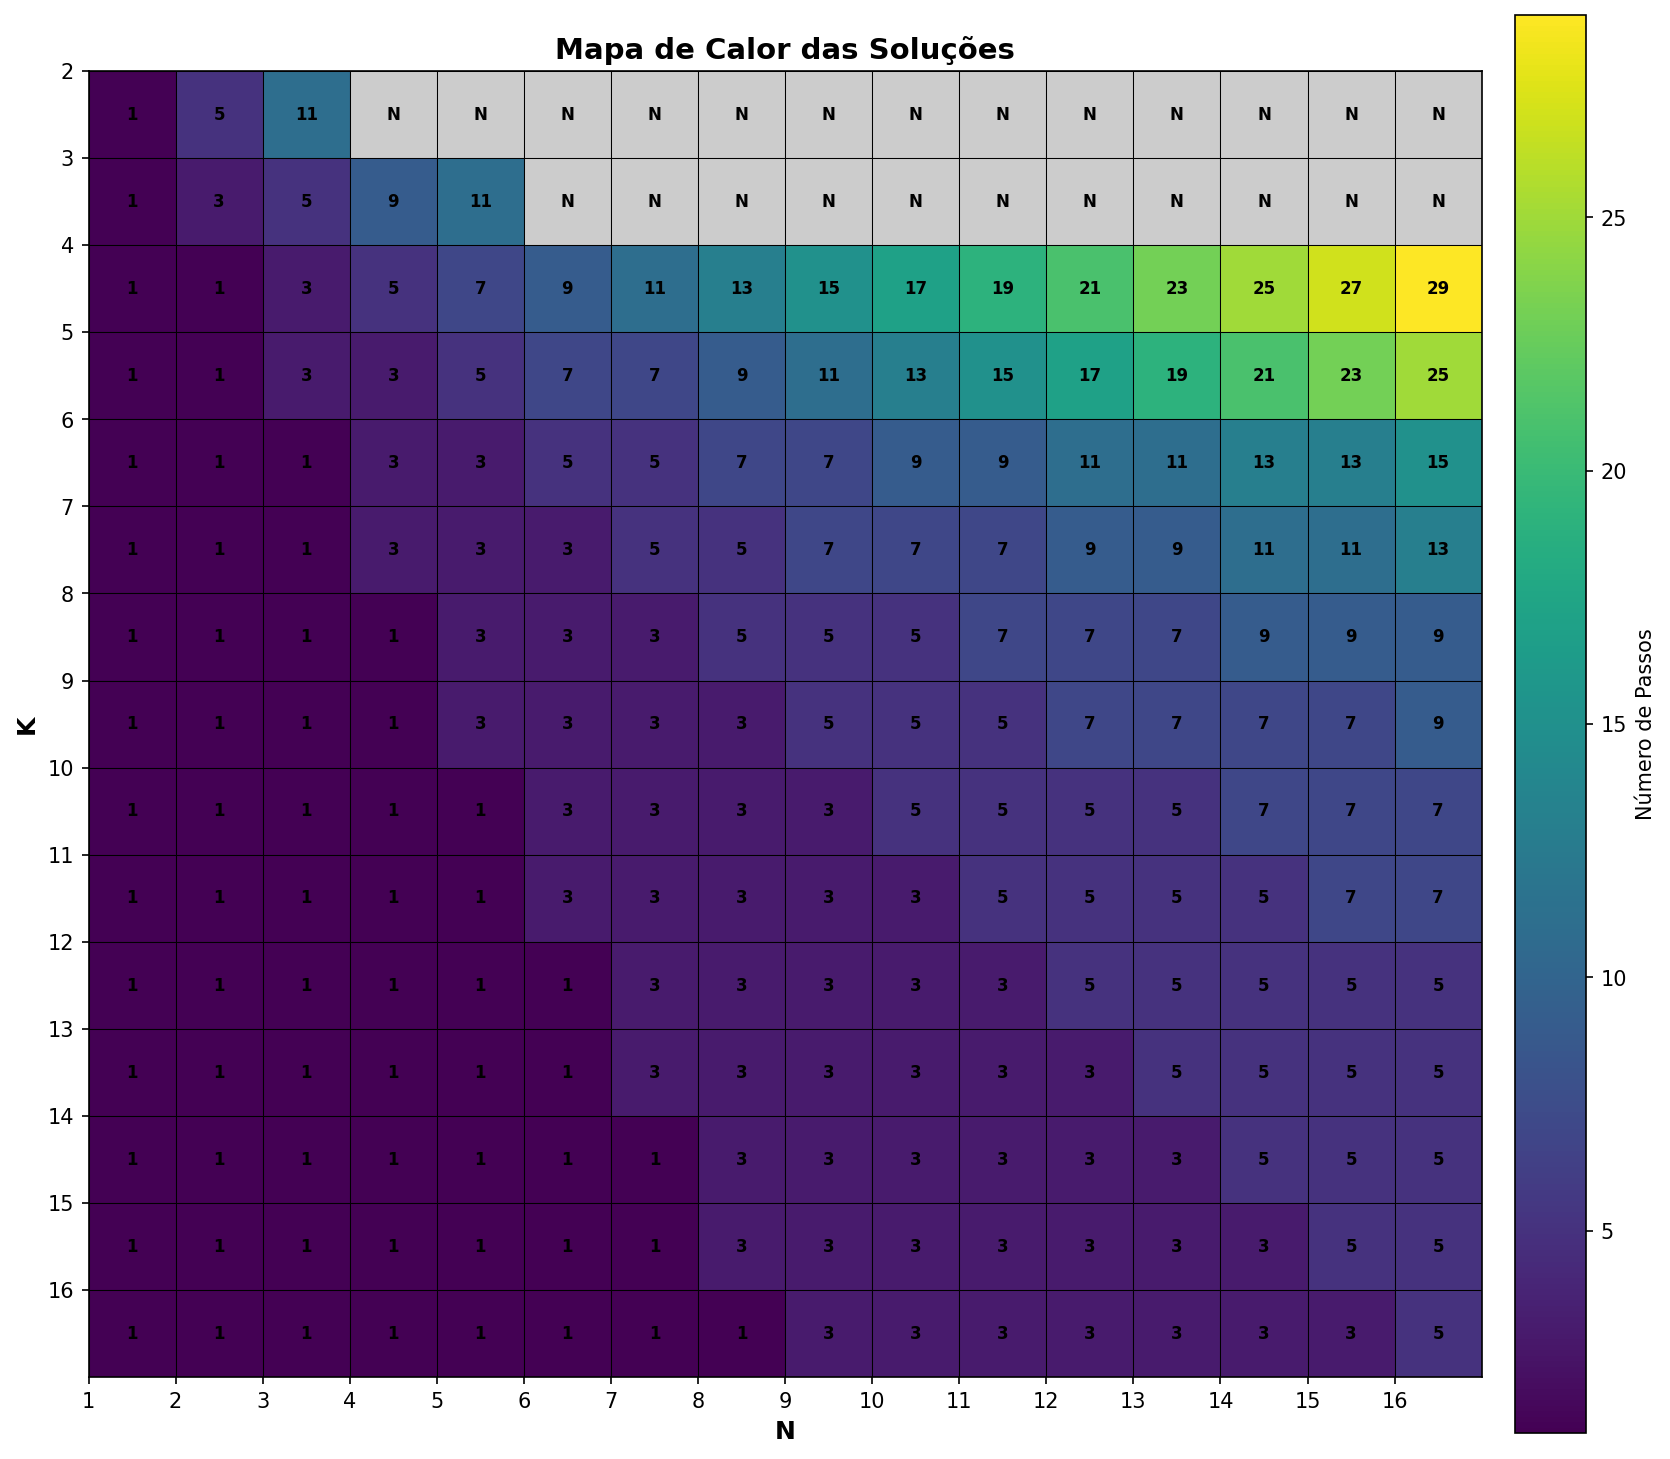
\includegraphics[width=0.9\textwidth]{solution_heatmap.png}
    \label{fig:heatmap}
\end{figure}

\subsection{Importância da deduplicação}
Para ilustrar o impacto da deduplicação, fixamos $N = 8$ e comparamos as execuções com $K \in \{4, 5, 6, 7, 8\}$, plotando o número acumulado de estados explorados no eixo Y conforme a profundidade avança no eixo X. A Figura \ref{fig:explored_states_vs_depth} apresenta esse resultado, apresentando a execução sem deduplicação no painel esquerdo e a execução com deduplicação no painel direito.

A hipótese central é que barcos menores produzem soluções mais profundas, mais idas e vindas são necessárias para atravessar todos, enquanto barcos maiores produzem soluções rasas, mas com maior fator de ramificação em cada nível. Sem deduplicação, os estados repetidos se acumulam exponencialmente em ambos os casos, tornando a busca intratável mesmo para N moderados. Com deduplicação, o número de estados únicos é limitado pela cardinalidade do espaço de estados.

\begin{figure}[H]
    \centering
    \caption{Comparação do número de estados explorados em função da profundidade da busca, com e sem deduplicação.}
        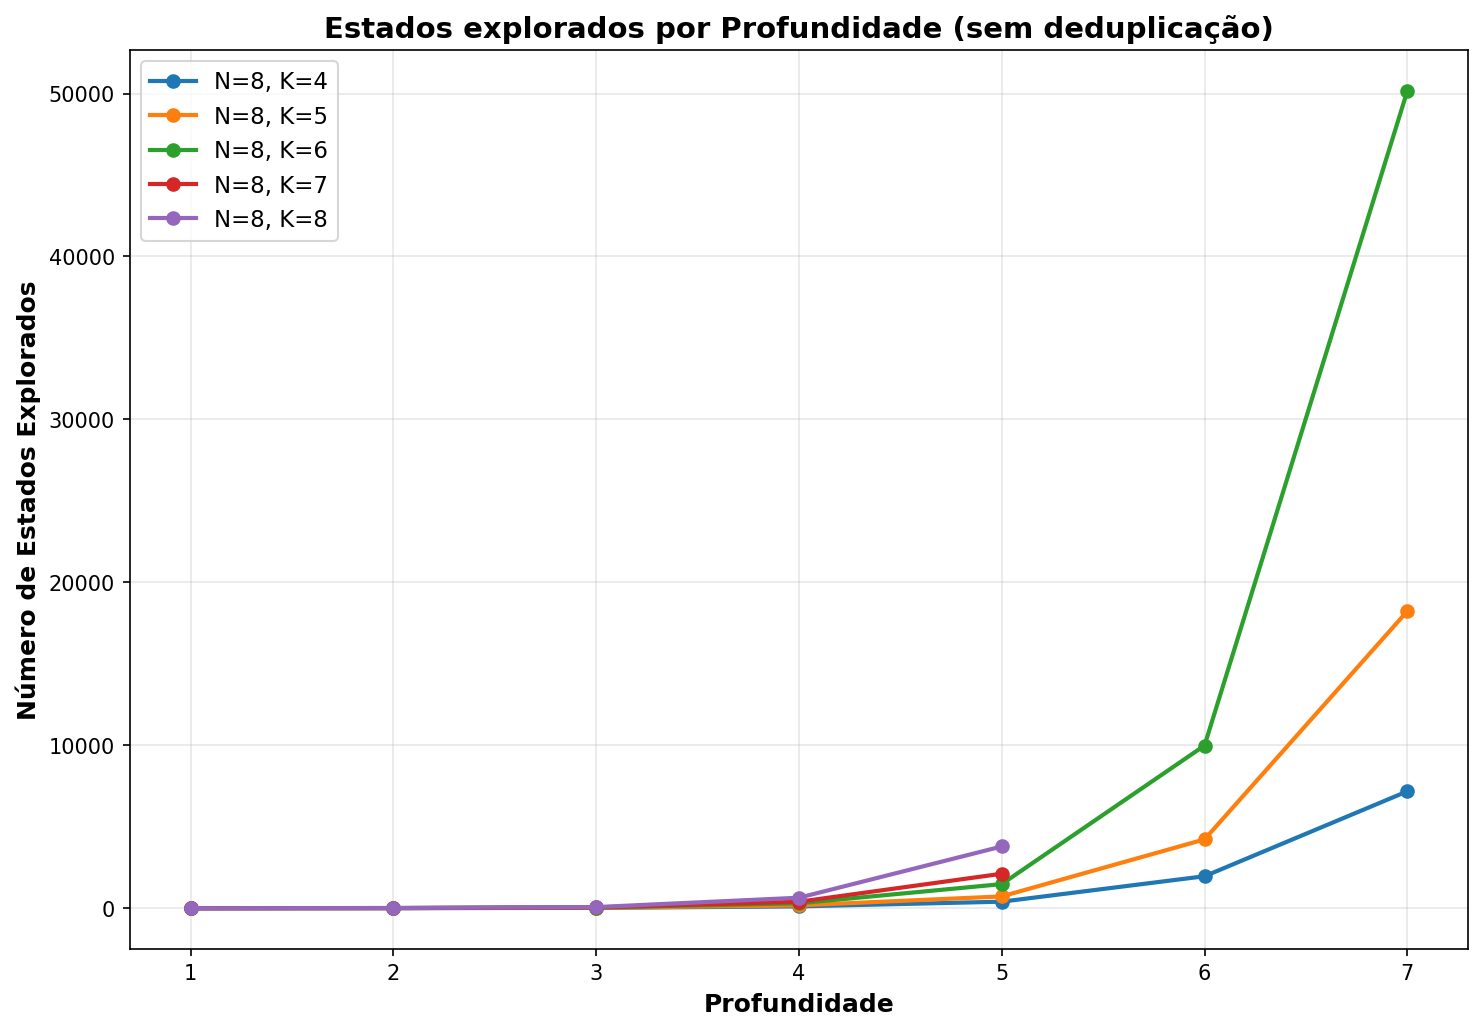
\includegraphics[width=0.45\textwidth]{explored_states_vs_depth_d0.png}
        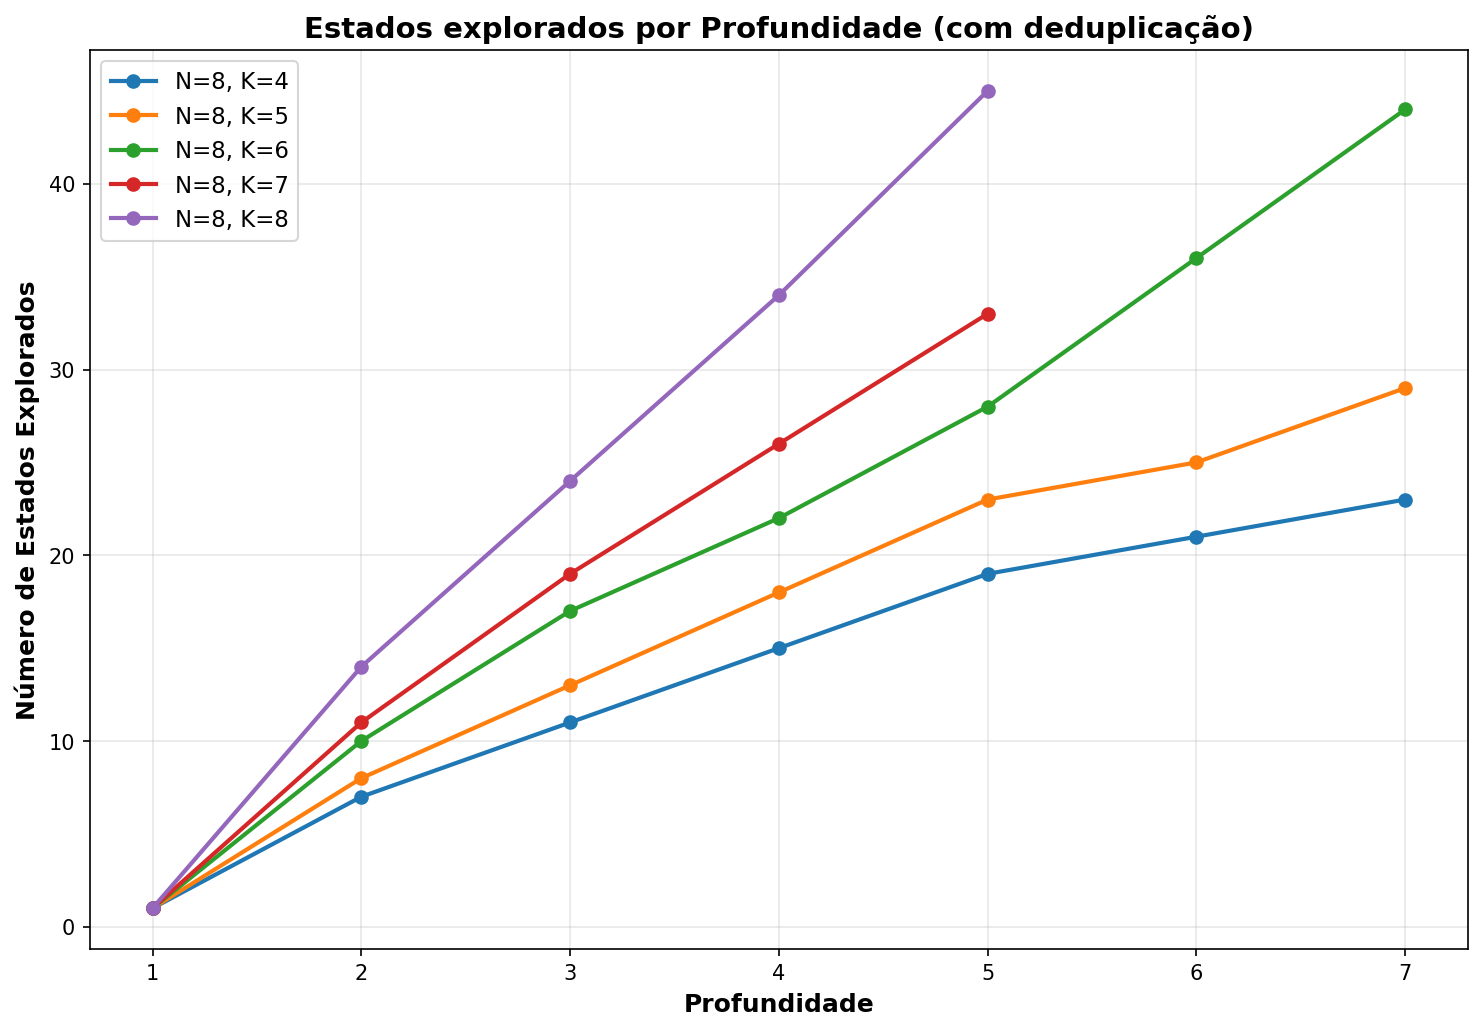
\includegraphics[width=0.45\textwidth]{explored_states_vs_depth_d1.png}
    \label{fig:explored_states_vs_depth}
\end{figure}

Sem deduplicação, o número de estados cresce de forma acentuada a cada nível da árvore, pois os mesmos estados são reenfileirados repetidamente através de caminhos distintos. Com deduplicação, as curvas crescem de forma muito mais contida e convergem rapidamente, refletindo o fato de que o espaço de estados únicos é finito. Esse contraste justifica a adoção obrigatória da tabela \textit{hash} em qualquer execução prática, uma vez que, além de reduzir o consumo de memória e tempo, ela é a única garantia de terminação nos casos sem solução.

A Figura \ref{fig:stacked_states_per_depth} mostra a proporção de estados explorados e ignorados em função da profundidade para $N=64$ e $K=32$. Pode-se observar que a deduplicação é bem eficiente, pois faz com que o algoritmo não explore desnecessariamente estados já vistos.

\begin{figure}[H]
    \centering
    \caption{Proporção de estados explorados e ignorados em função da profundidade}
        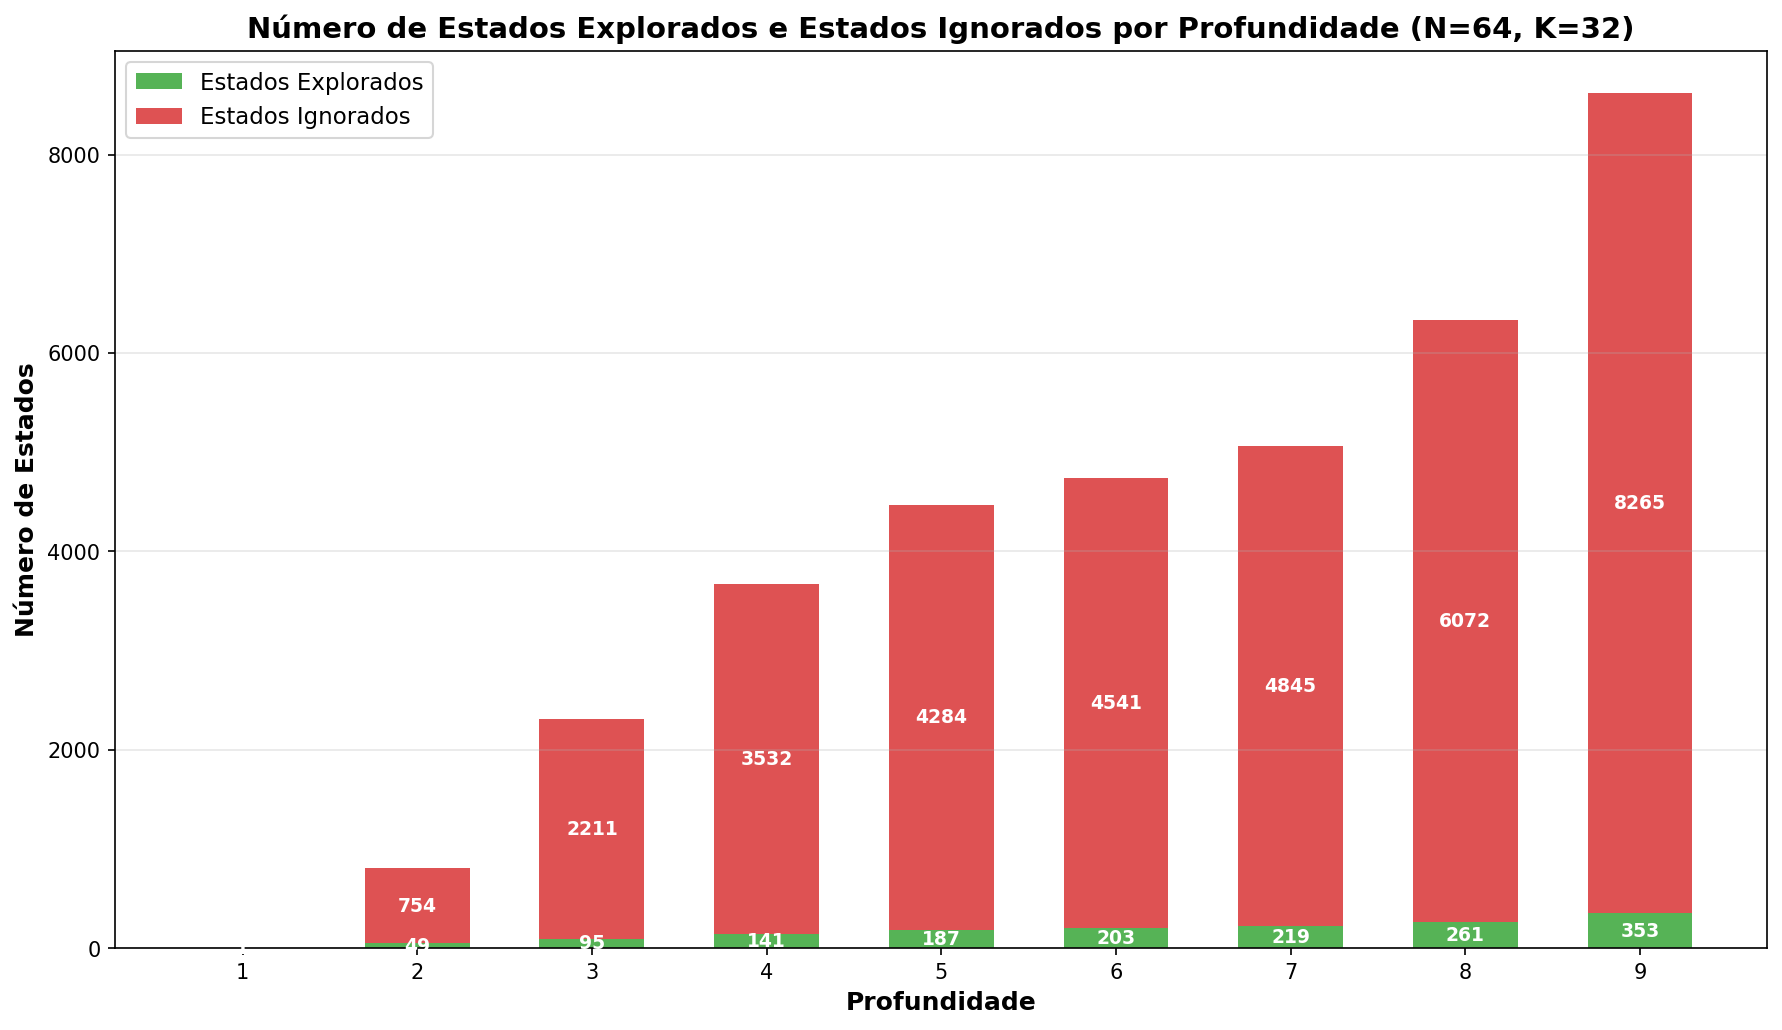
\includegraphics[width=0.6\textwidth]{stacked_states_per_depth_n64_k32.png}
    \label{fig:stacked_states_per_depth}
\end{figure}


\subsection{Desempenho em função de N}

Para avaliar como a complexidade escala com o tamanho do problema, fixamos alguns valores representativos de $K$ e variamos $N$ no eixo X, plotando o tempo de execução e a memória de pico no eixo Y. A memória de pico é extraída do maior valor de \textit{memory usage} reportado durante a execução.

Como a Figura \ref{fig:time_memory_vs_n_by_k} mostra, há um crescimento aparentemente linear da memória à medida que o $N$ aumenta para um mesmo $K$, e um crescimento aparentemente linear do tempo.

\begin{figure}[H]
    \centering
    \caption{Complexidade de tempo e de memória em função de N}
        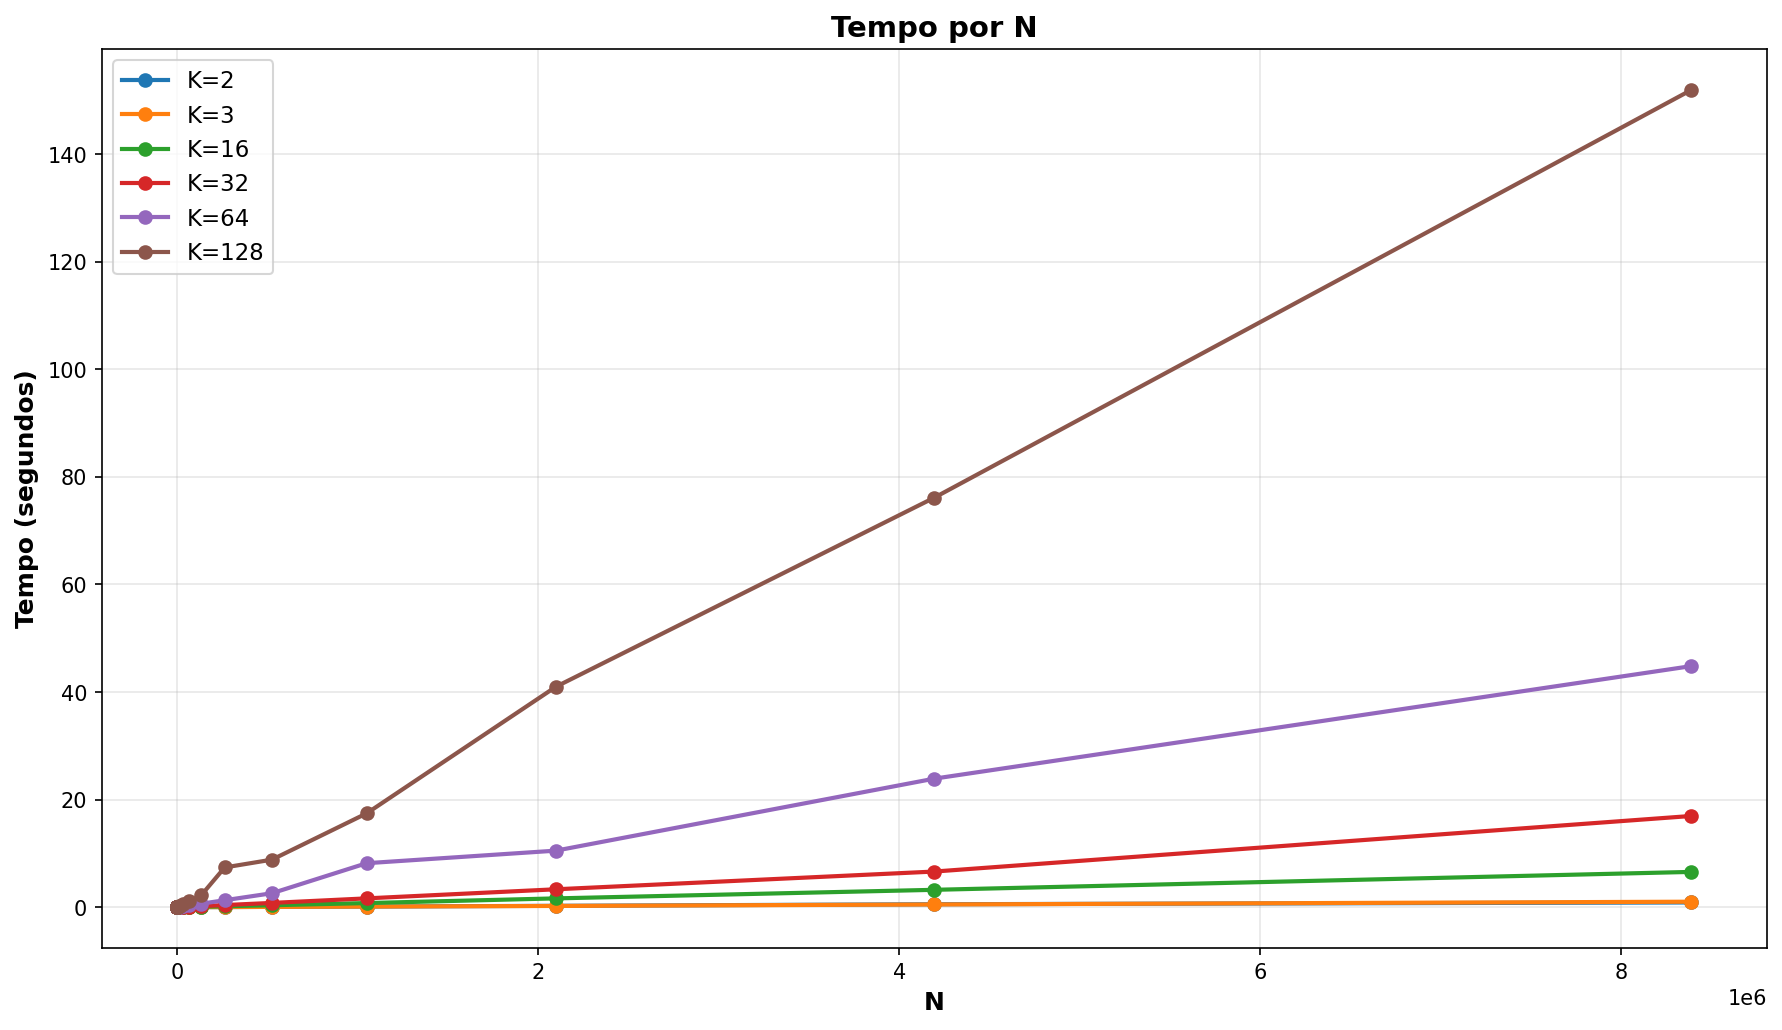
\includegraphics[width=0.45\textwidth]{time_vs_n_by_k.png}
        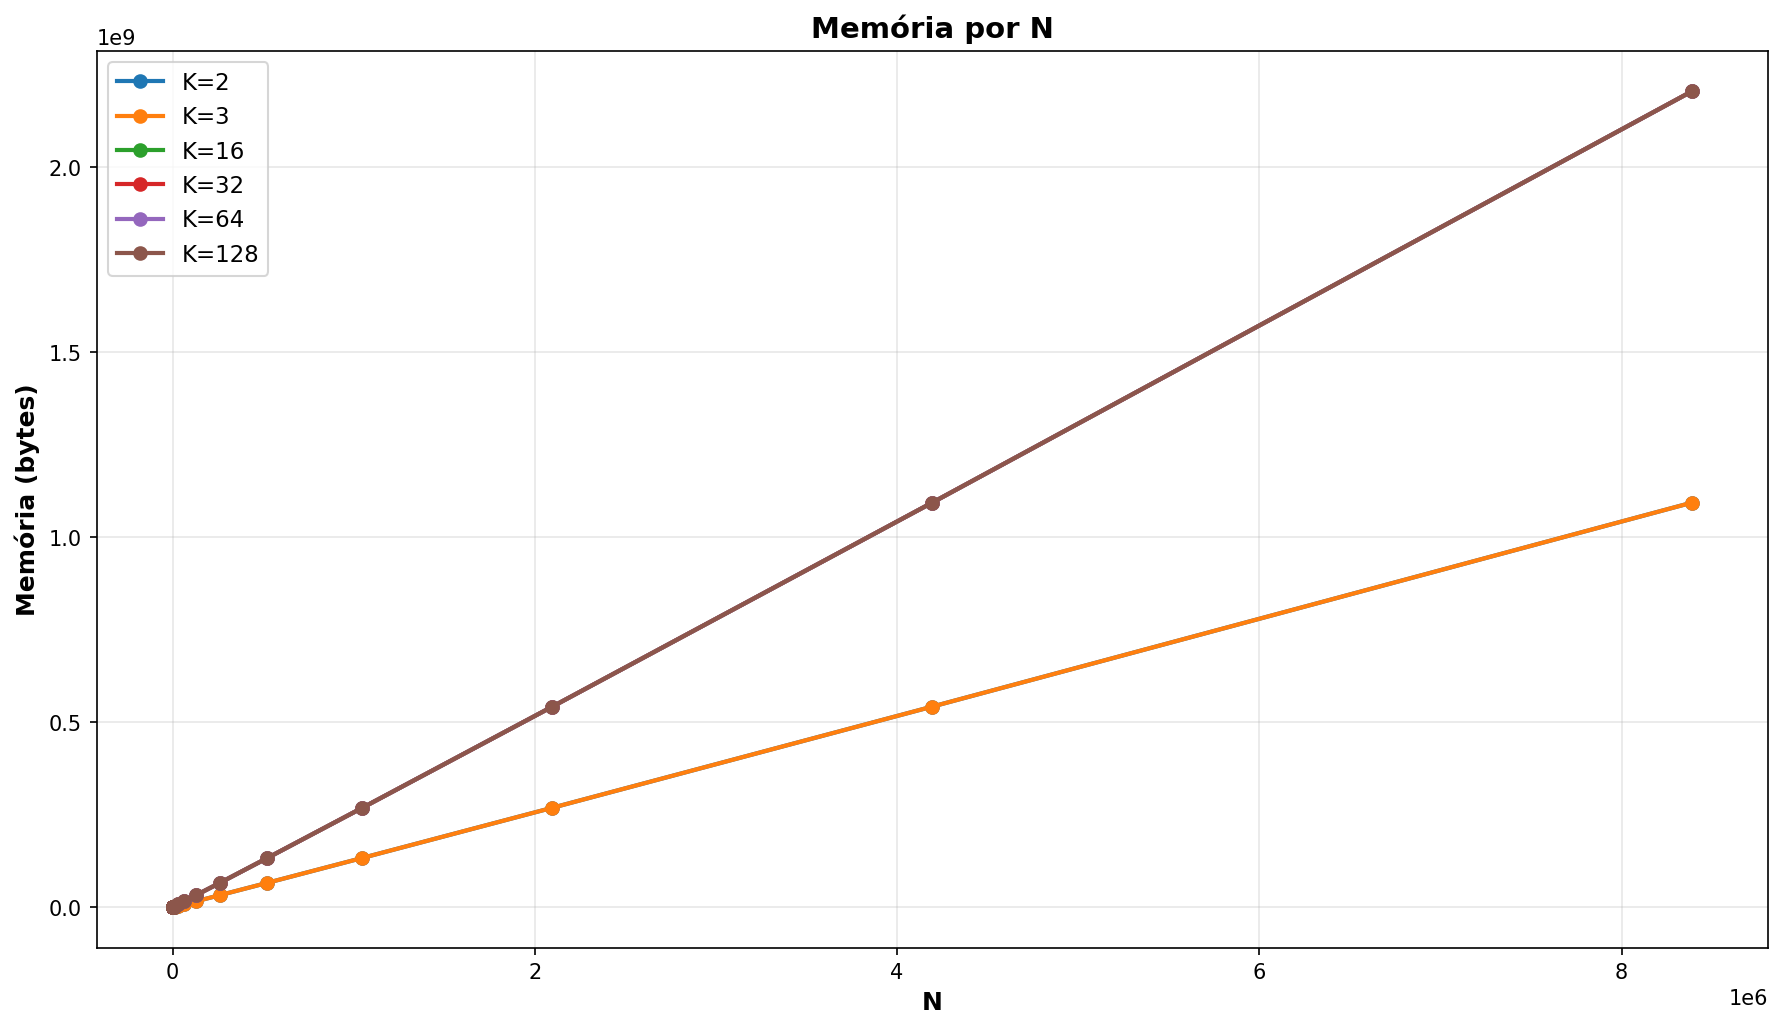
\includegraphics[width=0.45\textwidth]{memory_vs_n_by_k.png}
    \label{fig:time_memory_vs_n_by_k}
\end{figure}

Observa-se que conforme esperado, tanto a memória, quanto o tempo de execução crescem à medida que o $N$ também cresce para um mesmo $K$. Isso mostra que é necessário mais viagens de barco para resolver o problema, uma vez que temos mais passageiros.

A Figura \ref{fig:memory_vs_n_by_k_limited} mostra com mais detalhes, para $N$ limitado entre $1$ e $256$, esse comportamento da memória conforme o $N$ aumenta.

\begin{figure}[H]
    \centering
    \caption{Complexidade de memória em função de N limitado entre 1 e 256}
        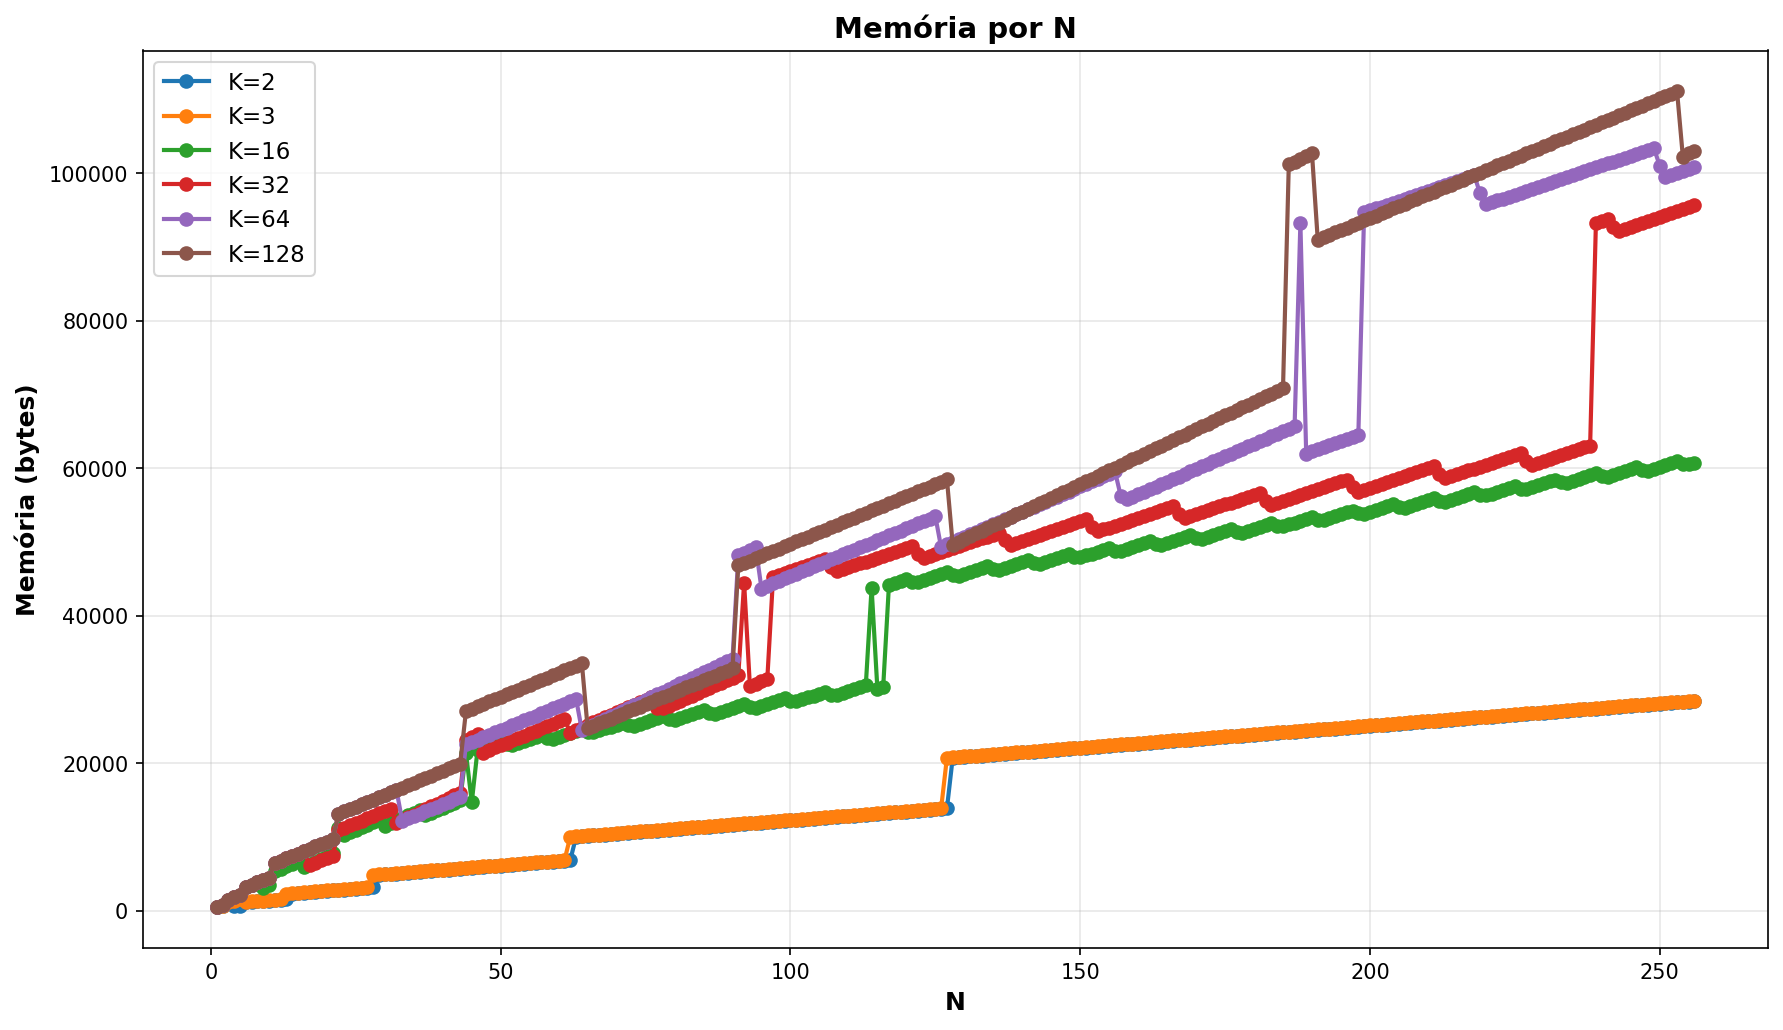
\includegraphics[width=0.6\textwidth]{memory_vs_n_by_k_limited.png}
    \label{fig:memory_vs_n_by_k_limited}
\end{figure}

\subsection{Desempenho em função de K}

Para estudar o efeito isolado da capacidade do barco, fixamos valores representativos de $N$ e variamos $K$ no eixo $X$.

O comportamento do tempo de execução mostra um crescimento aparentemente exponencial no tempo de execução para um mesmo $N$ à medida que o $K$ aumenta, ou seja, quanto maior $K$, maior a ramificação da árvore, e precisa-se de mais tempo para percorrer sua largura, como pode ser visto na esquerda da Figura \ref{fig:sankey}.

Nota-se que o pico da memória depende apenas do valor de $N$ a partir de certo valor, mas que inicialmente, com valores de $K$ pequenos, cresce rapidamente á medida que o $K$ aumenta, depois mantendo a constância aparente na direita da Figura \ref{fig:sankey}.

\begin{figure}[H]
    \centering
    \caption{Complexidade de tempo e memória em função de K}
        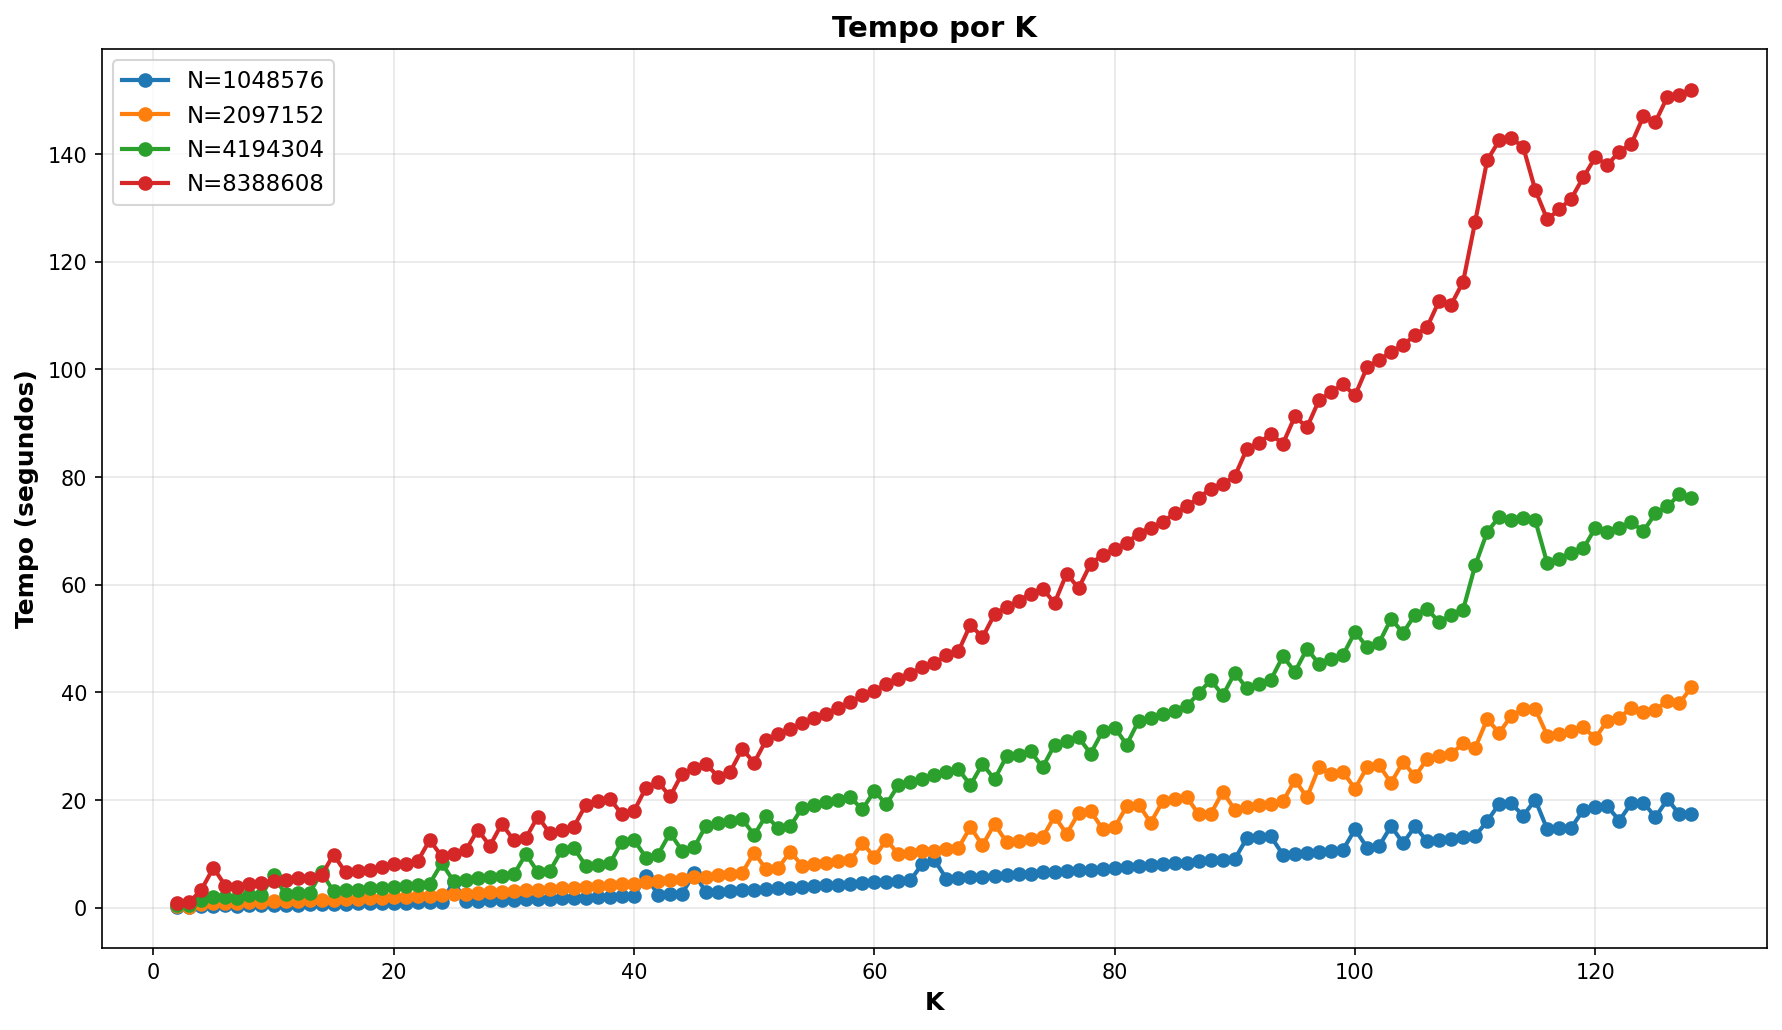
\includegraphics[width=0.45\textwidth]{time_vs_k_by_n.png}
        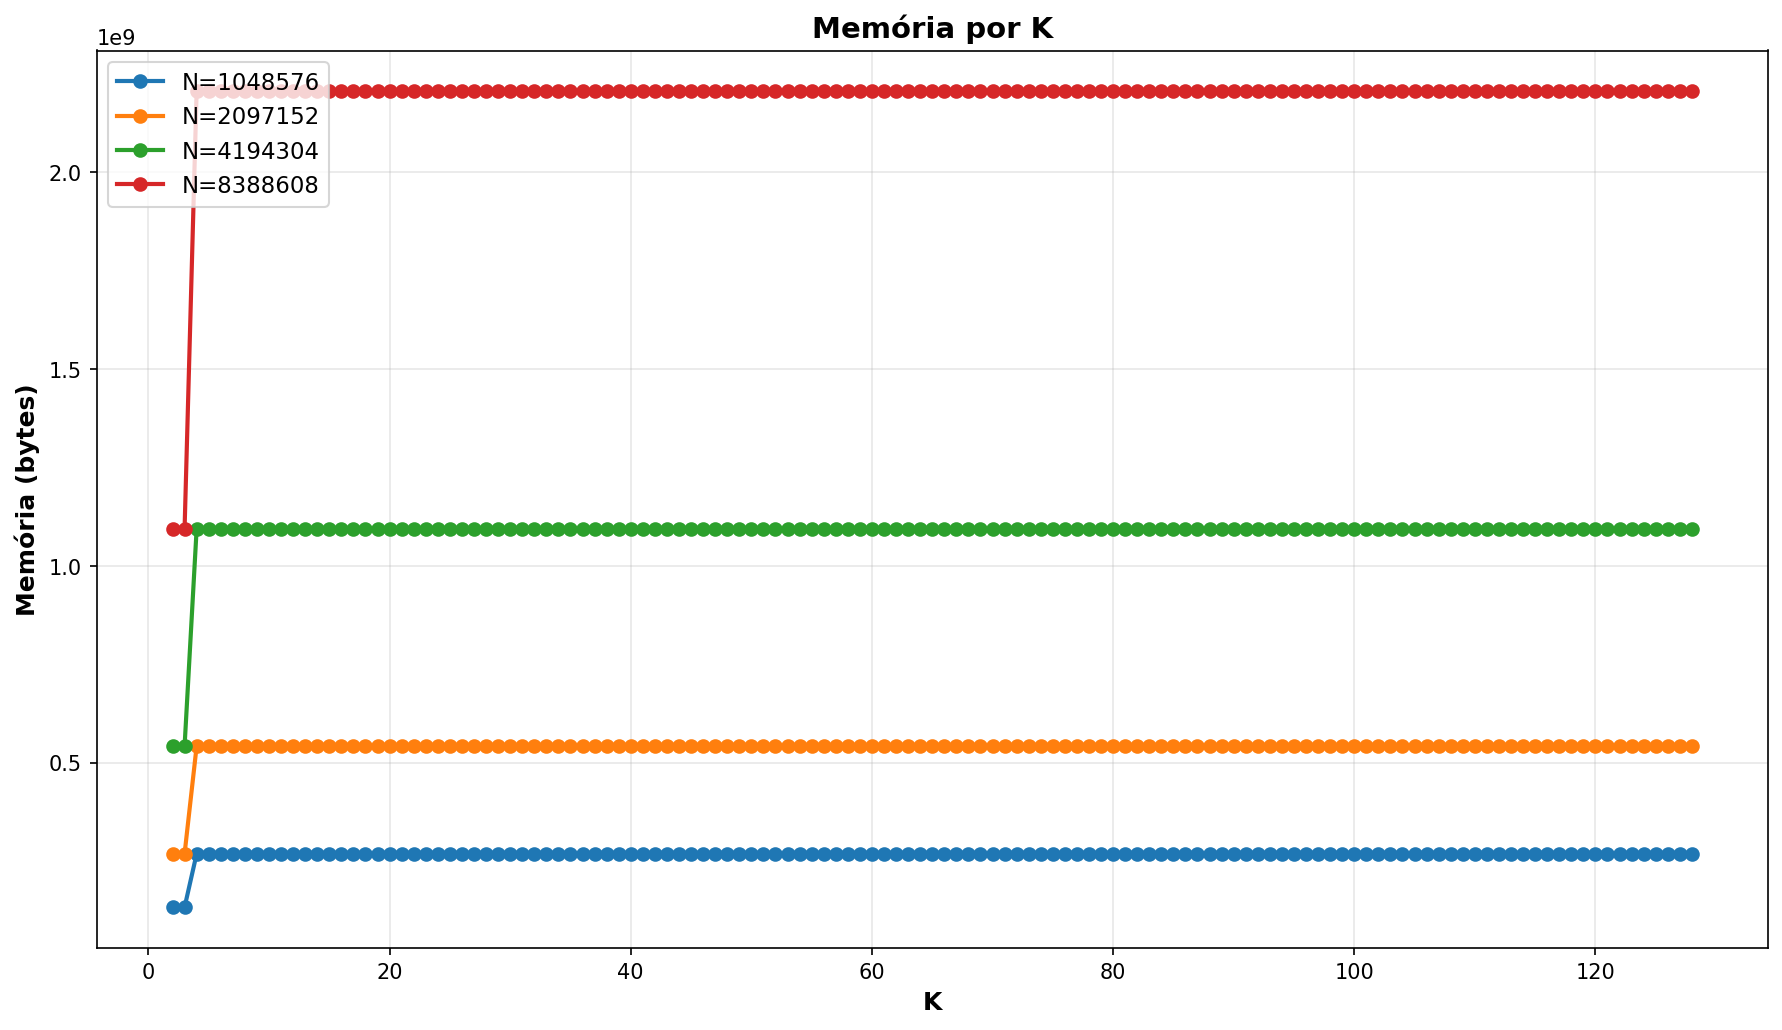
\includegraphics[width=0.45\textwidth]{memory_vs_k_by_n.png}
    \label{fig:sankey}
\end{figure}


\section{Conclusão}

Esse trabalho teve como objetivo generalizar o problema clássico dos canibais e missionários parametrizando o tamanho do barco e a quantidade de personagens. A abordagem com BFS se mostrou eficiente para encontrar a soluções ótimas com o mínimo de travessias. Os principais achados podem ser sintetizados por:
\begin{itemize}
    \item A deduplicação via tabela \textit{hash} se mostrou indispensável, sem ela o algoritmo se torna impraticável para $N$ moderados e não há garantia de terminação em casos sem solução.
    \item O tempo e a memória crescem aparentemente de forma linear com $N$ para $K$ fixo.
    \item O aumento de $K$ tem impacto mais agressivo no tempo acarretando em um crescimento aparentemente exponencial, pois amplia o fator de ramificação da árvore de busca.
    \item A memória satura a partir de certo $K$, passando a depender predominantemente de $N$, o que sugere que o espaço de estados únicos é limitado pela cardinalidade do espaço e não pela ramificação.
\end{itemize}


\end{document}

